\documentclass[10pt]{IETBook}
\usepackage{color,soul}
\begin{document}

%For RH Book title
\rhbooktitle{DC Distribution Systems and Microgrids}

\markboth{DC Distribution Systems and Microgrids}{Demonstration Sites of DC Microgrids}

\cauthor{Laura~Ram\'{i}rez-Elizondo\thanks{Delft University of Technology}
Seyedmahdi~Izadkhast\thanks{Delft University of Technology} 
Aditya~Shekhar\thanks{Delft University of Technology} and
Pavol~Bauer\thanks{Delft University of Technology}}

\chapter{Demonstration sites of DC microgrids}

Write a paragraph introducing the topic and what is to come in the next sections.

\section{Off Grid Sites}
Here, we show the pilot projects undergoing in developing nations and remote locations with dc based energy distribution.
\subsection{Japan}
Work by Annette Wert and Kenji Tanaka can find mention here.
\subsection{India}

48 V dc stand alone examples are available. One of the examples is Jhunjhunwala, IIT Chennai.

\subsection{Bangladesh}
\subsection{More locations?}
\section{Transportation Electrification}
Electrification of the transportation sector is driven by the desire to shift towards clean energy sources and reduced emissions. DC based energy sharing in subsystems of electric vehicles, ships, trains and airplanes is finding traction as the component integration is much more efficient and compact. Considering that most loads are energy intensive, efficiency becomes important. The potential size and weight reduction is an even more critical pivot towards adopting dc in transport systems.

Since the elements of transportation sector are inherently standalone, the market inertia of ac systems can be bypassed, making it easier for dc to make inroads. Consequently, it is observed that pilot demonstrations and commercial penetration of dc microgrids in transportation electrification are significant. This section provides an overview of such initiatives across the world.
\subsection{Shipboard DC Microgrids}
The interest in all electric ships (AES), fuelled by the need for efficient space utilization, has given rise to the concept of dc based integrated power system (IPS)~\cite{alb}. An illustration of such a dc microgrid island on ship is shown in Figure~\ref{shipillus}.
\begin{figure}[!h]
\centerline{\fbox{\hbox to 0.8\textwidth{\vbox to 16pc{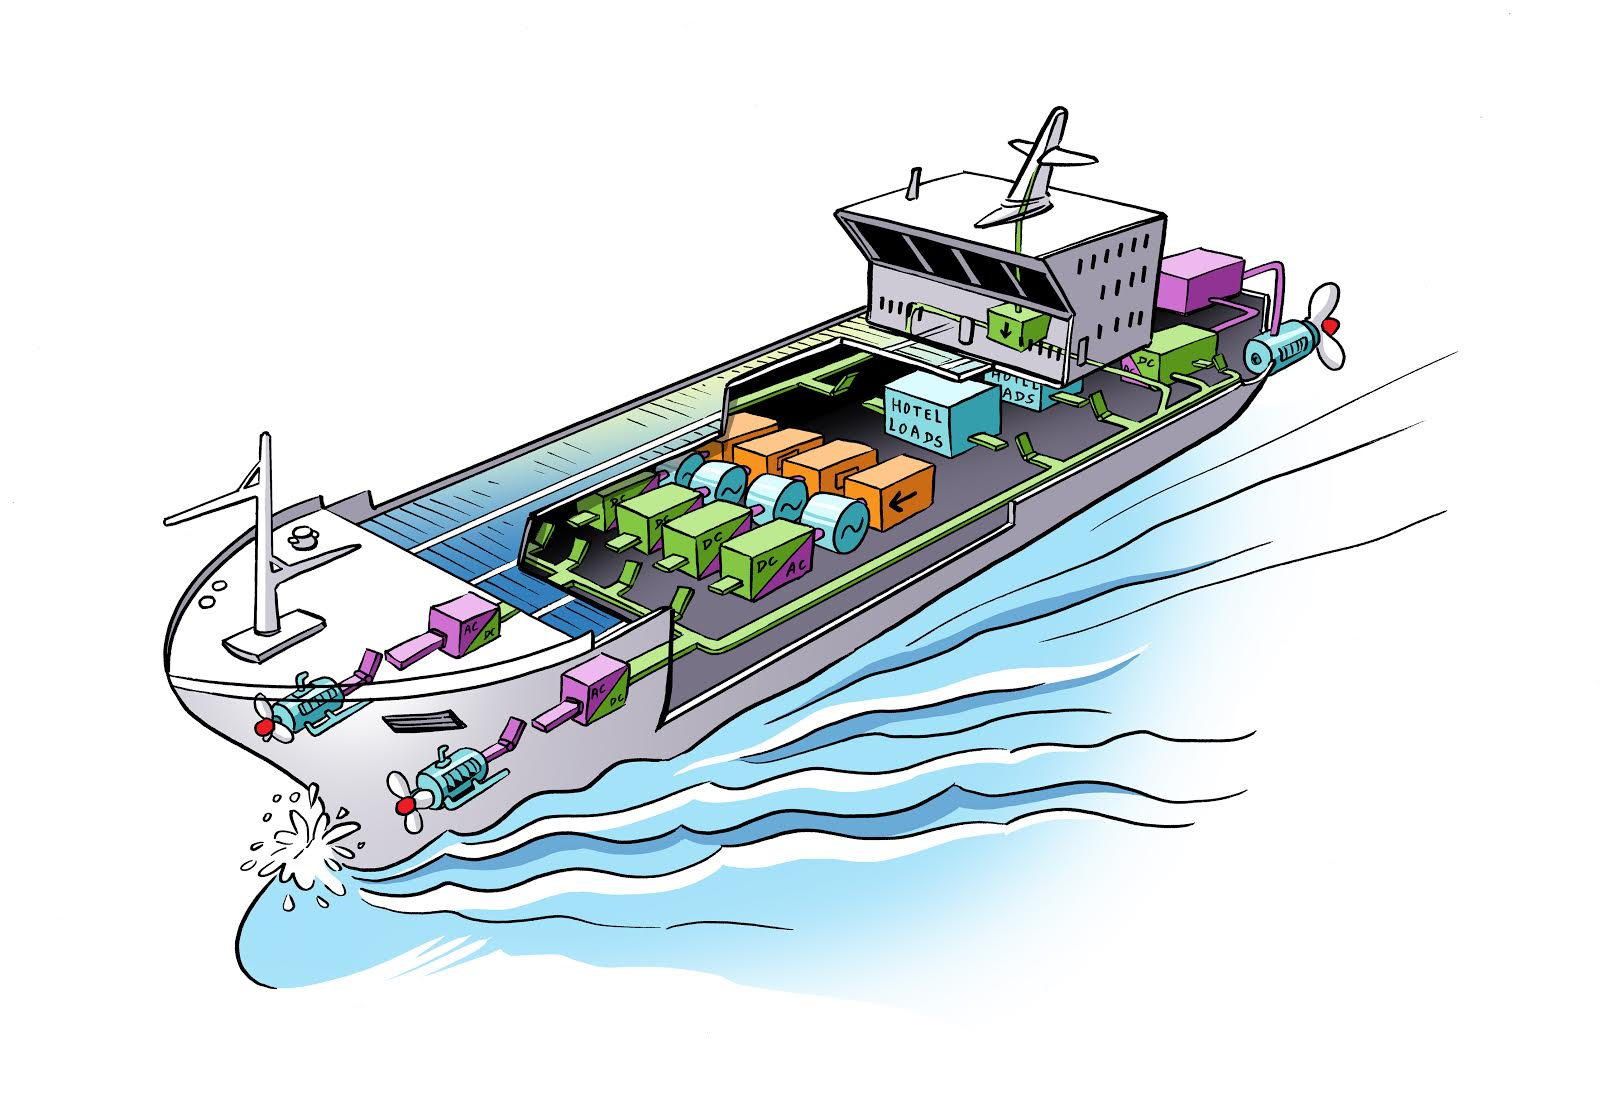
\includegraphics[width=0.9\textwidth]{images/ships}}}}}
\caption{An illustration of a dc-based all electric ship.}
\label{shipillus}
\end{figure}

The operating voltage levels are between 1\,kV to 35\,kV. The recommended practices for reliable integration of shipboard power components in a medium voltage dc (MVDC) system is discussed by the IEEE standards association~\cite{ieee}. 
\subsubsection{Architecture}
Keeping in mind the redundancy requirements, two buses, port and star board bus, run through the length of the ship. Relevant shipboard dc zonal electrical distribution system (ZEDS) architectures with tradeoffs between reliability, complexity and efficiency are discussed in~\cite{alb}. Herein, the so-called \lq \lq Dual-ring-bus\rq \rq dc ZEDS is described. It is identified that due to inter-connectivity, the reconfiguration capability during contingencies maybe a potential advantage of MVDC IPS in AES. Extensive use of solid state circuit breakers is employed. The sequential self healing system reconstruction when 3 faults occur is shown in Figure~\ref{figalb}.
\begin{figure}[!h]
\centerline{\fbox{\hbox to 0.95\textwidth{\vbox to 14pc{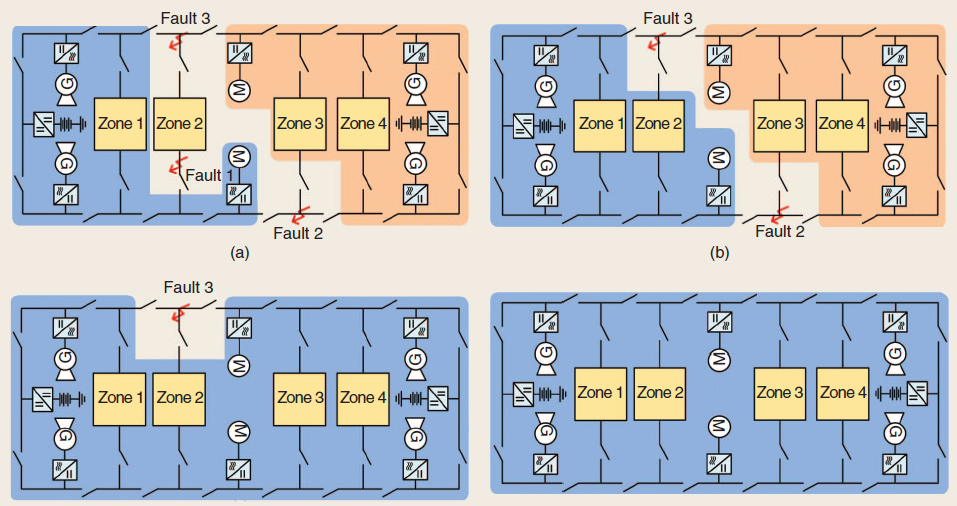
\includegraphics[width=0.95\textwidth]{images/reconship}}}}}
\caption{Reconfigurable system architecture for a general dc shipboard power system: (a) Faults occur (b) Fault 1 clear (c) Fault 2 clear (d) Fault 3 clear (courtesy:~\cite{alb}).}
\label{figalb}
\end{figure}
\subsubsection{Testbeds in United States of America}
The U.S. office of Naval Research created a consortium of seven universities for Electric Ship Research and Development (ESRDC)~\cite{usuninavy}. When it was renewed for the term 2007-12, some of its thrusts were the design of ship electric power system and next generation IPS. Towards this goal, the ESRDC team planned to develop a MVDC distribution demo with navy resources.

As part of this consortium, the University of Texas at Austin center for electromechanics (UT-CEM) assembled a MVDC microgrid at MW level~\cite{austin}. The key components of the developed testbed along with the actual setup images are shown in Figure~\ref{figaustin}. The objective was to experimentally validate the system models and demonstrate the critical issues in the naval electrical system.
\begin{figure}[!h]
\centerline{\fbox{\hbox to 0.9\textwidth{\vbox to 19pc{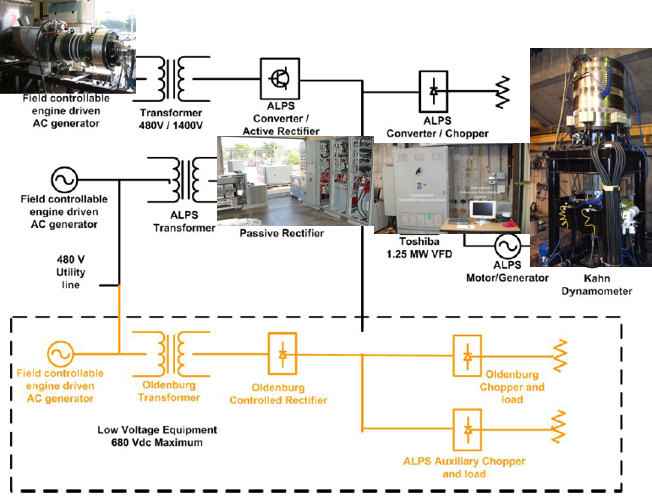
\includegraphics[width=0.9\textwidth]{images/austin}}}}}
\caption{Flexible testbed at UT-CEM for MVDC shipboard microgrid (adapted from~\cite{austin}).}
\label{figaustin}
\end{figure}

The isolated naval microgrid is envisioned to operate at 80 to 100\,MW with different steady state and pulsed power loads. UT-CEM microgrid demonstrator is a flexible testbed as its power level can be expanded by several MW, the operating voltage levels can be redefined and the entire system can be reconfigured. During the publication of the paper~\cite{austin}, the system was operating at 2\,kV dc at a bus which physically spanned 150\,ft within the lab. While the reported focus was on series faults, the following research demonstrations were planned:
\begin{itemize}
    \item Transients associated with microgrid islanding and reconnection.
    \item Ancillary services with different control strategies for better power quality.
    \item Effective fault management and protection. 
    \item Behaviour of the microgrid with pulsed power load, which maybe critical for military ships.
    \item Integration of storage elements.
\end{itemize}

Another ESRDC partner, Massachusetts Institute of Technology, Cambridge, USA, is developing the physical concept of "Power Corridor" towards the IPS keeping in mind the space reservations for AES~\cite{mit}. A MVDC fault management testbed for ship power system is the focus of Florida State University~\cite{fsu}. A complete description of the initiatives and progress of the entire ESRDC consortium is beyond the scope of this discussion.
\subsubsection{Testbeds in Europe}
Some initiatives on shipboard IPS with MVDC microgrid have also been taken in Europe. For instance, the University of Trieste in Italy conceived a 2\,MVA, 22500 rpm, 12 phase permanent magnet  prototype generator~\cite{sulli}, connected to 3\,kV dc IPS with a controlled active ac-dc converter as shown in Figure~\ref{figsulli}. This program aimed at obtaining experimental results for shipboard MVDC IPS for naval applications. 
\begin{figure}[!h]
\centerline{\fbox{\hbox to 0.9\textwidth{\vbox to 17pc{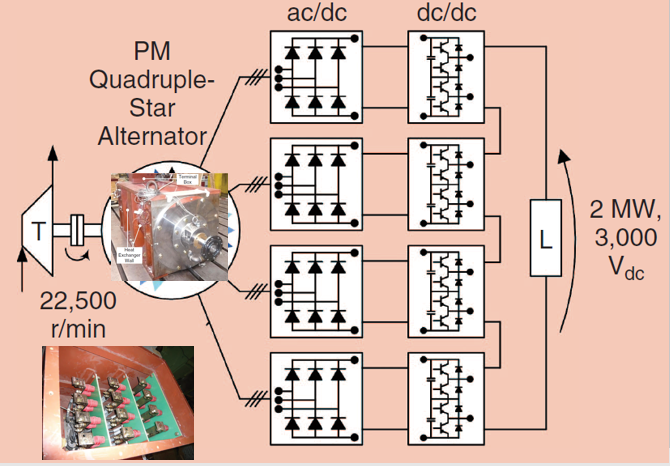
\includegraphics[width=0.9\textwidth]{images/gensyst}}}}}
\caption{A prototype generation system a shipboard medium voltage dc integrated power system adapted (adapted from~\cite{sulli}).}
\label{figsulli}
\end{figure}

This was an advanced version of a previous 6300 rpm alternator connected to the dc bus with uncontrolled ac/dc converter. By raising the speed of the machine, a higher power density was achieved, thereby enabling a direct coupling with the gas turbine. Also, the weight of generator was reduced to less than 50\,\% of its predecessor, which is one of the key advantages of decoupling the speed limit of the generator from the operating grid frequency. 

The bus connected choppers were responsible for the output voltage control. The machine reacted to the power electronics and resulted in distortion in phase current, leading to flux pulsations and eddy current losses. This challenge was an important constraint towards the design choices. Noting that the prototype matched the expected requirements, the test results concluded that significant power density targets can be achieved by raising the generator speed.
\subsubsection{Commercial Realization}
The interest in onboard dc to eliminate ac switchboards, some power conversion stages and remove the need for bulky transformers led to the commercial design of Dina Star by ABB~\cite{abb1}. It was claimed that use of 1\,kV dc with upto 20\,MW demand improves the vessel's energy efficiency by 20\,\% and the weight of electrical system by 30\,\% ~\cite{abbart,abb0}.
\begin{figure}[!h]
\centerline{\fbox{\hbox to 0.9\textwidth{\vbox to 10pc{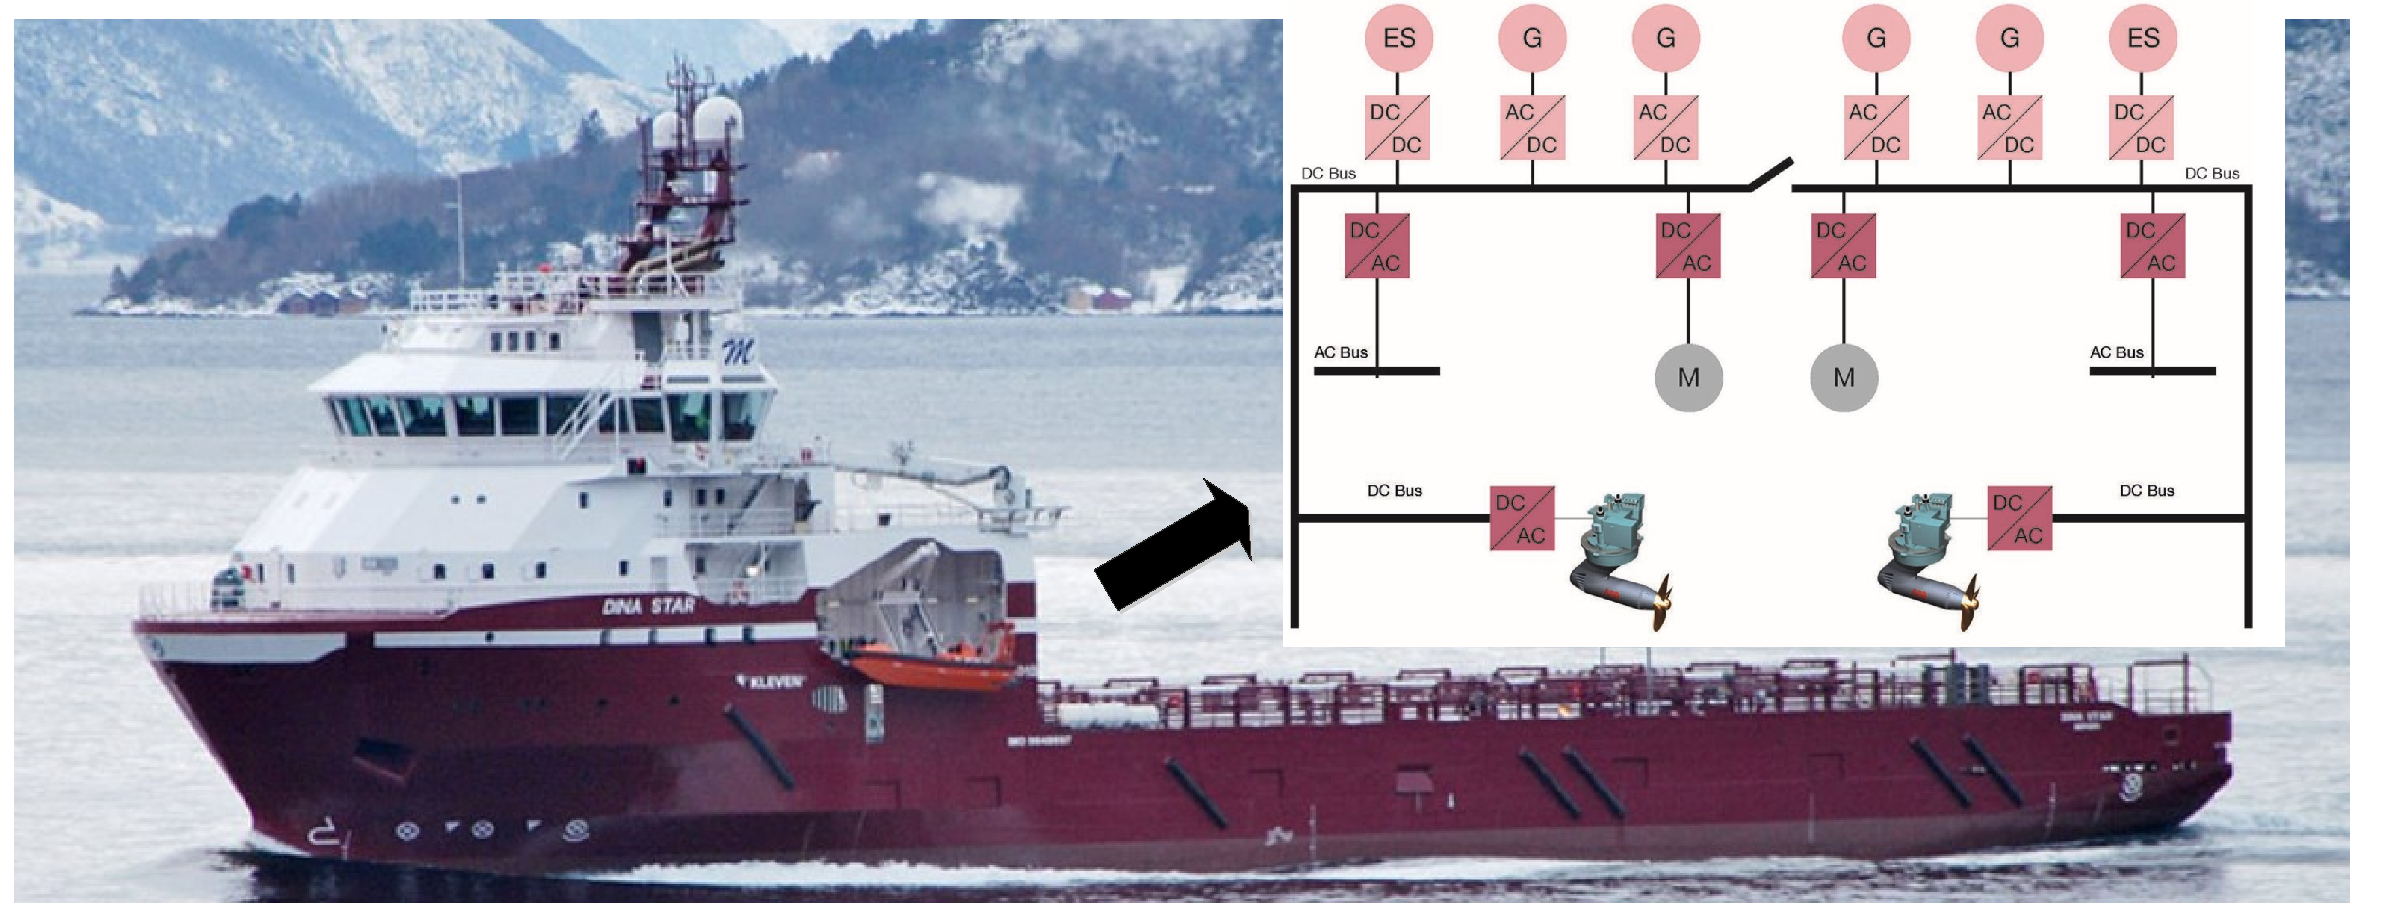
\includegraphics[width=0.92\textwidth]{images/dina}}}}}
\caption{ABB's Dina Star Ship with Onboard DC Grid  (adapted from~\cite{abb1}).}
\label{figdina}
\end{figure}

While acknowledging these significant efficiency gains and lesser problems with harmonic distortion, the challenge in the design of the marine on-board dc system was noted to be selectivity and protection. ABB made use of power electronics and coordinated use of fuses and isolation switches to circumvent this problem. Further, the controlled thyristor rectifier connected to the generator played an added role of protection device. It was claimed that dc fault currents can be controlled within 10 to 20\,ms, providing a significant reduction in fault energy as compared to the conventional ac system.

One year into the operation of Dina Star, demonstration tests on fuel consumption and noise reduction were conducted on voyage from Scotland to Norway~\cite{abb1}. The comparision was made between fixed and variable speed operation. As much as 27\,\% efficiency gains can be achieved for 10\,\% load. Cumulatively, it was concluded that between 9 to 14\,\%  efficiency gain can be achieved with variable load.
\subsection{Traction}
16.5 Hz
\subsection{Electric Vehicles}

\section{Smart Cities}

\subsection{Residential Applications}
Many household equipments like television, refrigerator, computer, LED lighting, etc; emerging energy intensive consumers like electric vehicles (EVs) as well as sources like solar photovoltaic (PV) and storage elements are dc in nature. It is envisioned that if these are interconnected with a common dc bus to form a \lq \lq nanogrid\rq \rq \ supported by the main grid, the energy exchange would become more efficient. Lack of dc ready household devices in the market have hindered this concept from being fully realized. Nevertheless, the anticipated benefits have driven the need for practical proof of concept. This section explores some initiatives taken in this direction. A typical grid connected residential house with dc distribution system is shown in Figure~\ref{figresarchi}. 
\begin{figure}[!h]
\centerline{\fbox{\hbox to 0.9\textwidth{\vbox to 13pc{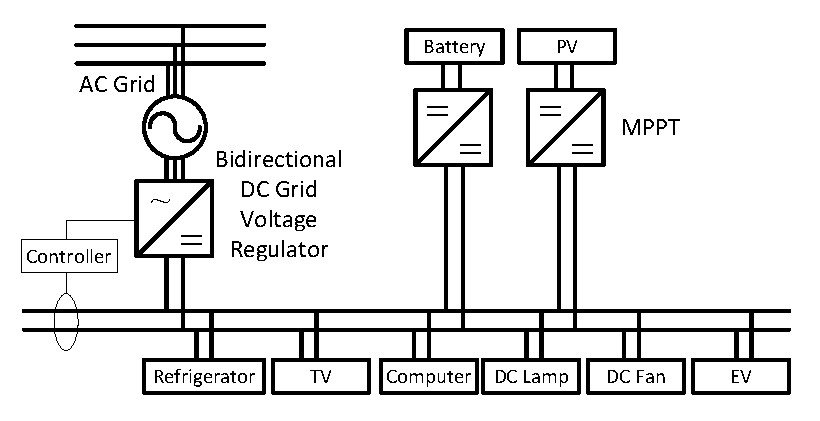
\includegraphics[width=0.9\textwidth]{images/dchome}}}}}
\caption{Grid connected residential microgrid.}
\label{figresarchi}
\end{figure}

For residential dc nanogrids, the common bus voltage appears to be standardizing around 380 $\pm$ 20\,V.~\cite{laurens,taiwandemo}. Heuristic controls try to minimize the energy exchange with the main grid using storage elements for operational efficiency while maximizing the distributed green energy resources in the system~\cite{taiwandemo}. The role of the bidirectional inverter (BDI) is to perform this energy balance, and consequently is responsible for voltage regulation. The role of BDI can be diversified, for example, to draw or store energy in the flywheel or operating it as a high power rating charger/discharger for dc UPS while reducing cost by designing the low power rating charger. The schematic for the latter is discussed in~\cite{taiwandemo} as shown in Figure~\ref{figbdi}.
\begin{figure}[!h]
\centerline{\fbox{\hbox to 0.61\textwidth{\vbox to 12pc{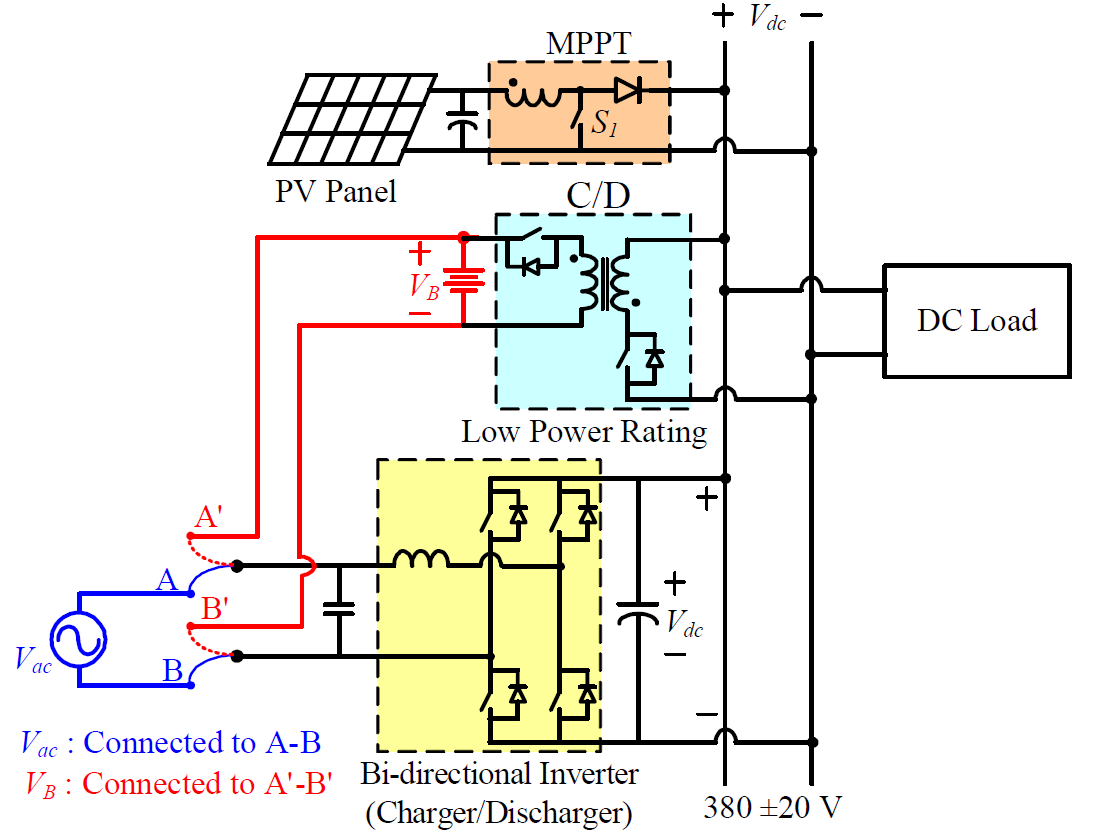
\includegraphics[width=0.6\textwidth]{images/bdi}}}}}
\caption{Dual role of bi-directional inverter in residential microgrid (courtesy:~\cite{taiwandemo}).}
\label{figbdi}
\end{figure}

\begin{figure}[!h]
\centerline{\fbox{\hbox to 0.9\textwidth{\vbox to 17pc{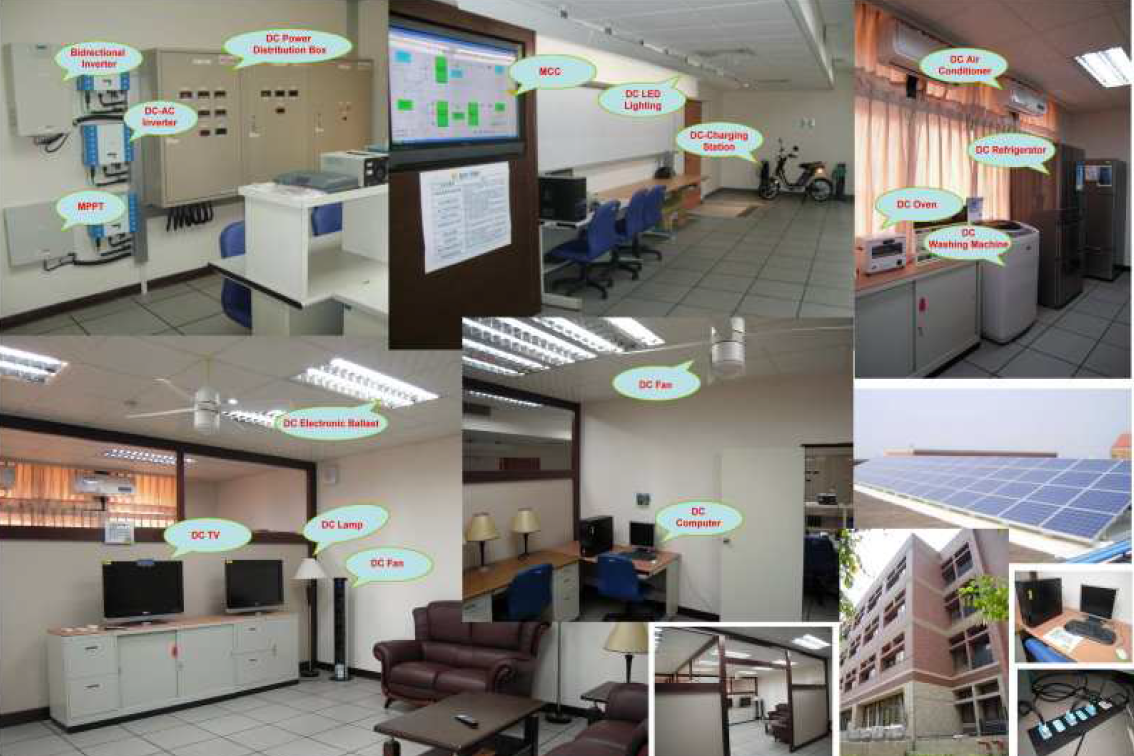
\includegraphics[width=0.9\textwidth]{images/taidemo}}}}}
\caption{Grid connected residential microgrid  (courtesy:~\cite{taiwandemo}).}
\label{figtaidemo}
\end{figure}
\subsection{Buildings and Workplaces}
\subsection{Campuses}
\subsection{EV - PV - Storage}
Mention here regarding tesla-solar city project.
\subsection{Big Data Application}

\section{Application Specific Examples}
\subsection{Data Centres}
\subsection{Street Lighting}
\subsection{Greenhouses}

\section{Testbeds}
Showcase some research initiatives by universities and research labs here.

\section{Societal Impact}
\section{Discussion}
\bibliographystyle{vancouver-modified}
\bibliography{sample-vancouver}

\end{document}
